\documentclass{oblivoir}
\usepackage{amsmath,amssymb,amsthm,kotex,mdframed,paralist,kswrapfig}

\newcounter{num}
\newcommand{\prob}
{\bigskip\noindent\refstepcounter{num}\textbf{보충문제 \arabic{num})}\par}

\newcommand{\ans}{{\raggedleft\textbf{답 : (\qquad\qquad\qquad\qquad\qquad\qquad)}
\par}\bigskip\bigskip}


%%%
\begin{document}
\Large

%
\prob
지수와 효정이는 바나나를 먹었습니다.
지수는 큰 바나나 2개를 먹었고 효정이는 작은 바나나 3개를 먹었습니다.
지수와 효정이가 먹은 바나나의 양을 가장 간단한 자연수의 비로 나타내세요.
(단, 큰 바나나의 크기는 작은 바나나의 크기의 두 배입니다.)

\begin{figure}[h!]
\centering
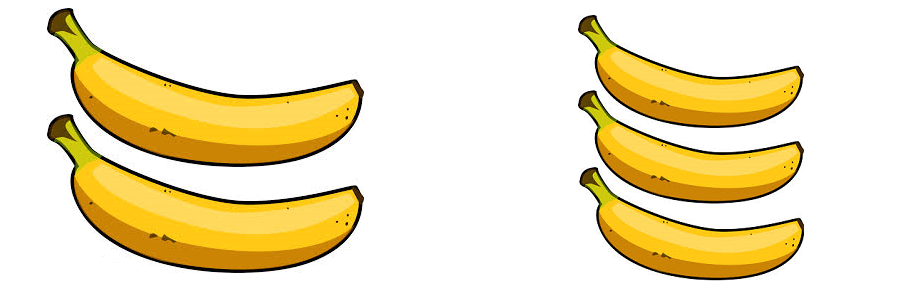
\includegraphics[height=0.15\textheight]{s01}

지수가 먹은 바나나 \qquad\qquad\quad 효정이가 먹은 바나나
\end{figure}

\ans


%
\prob
지수와 효정이는 바나나를 먹었습니다.
지수는 큰 바나나 3개를 먹었고 효정이는 작은 바나나 4개를 먹었습니다.
지수와 효정이가 먹은 바나나의 양을 가장 간단한 자연수의 비로 나타내세요.
(단, 큰 바나나의 크기는 작은 바나나의 크기의 두 배입니다.)

\begin{figure}[h!]
\centering
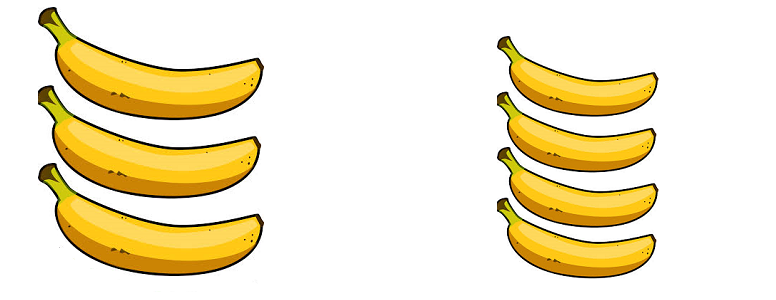
\includegraphics[height=0.21\textheight]{s02}

지수가 먹은 바나나 \qquad\qquad\quad 효정이가 먹은 바나나
\end{figure}

\ans

%
\prob
지수와 효정이는 바나나를 먹었습니다.
지수는 큰 바나나 1개와 작은 바나나 2개를 먹었고 효정이는 큰 바나나 2개와 작은 바나나 1개를 먹었습니다.
지수와 효정이가 먹은 바나나의 양을 가장 간단한 자연수의 비로 나타내세요.
(단, 큰 바나나의 크기는 작은 바나나의 크기의 두 배입니다.)

\begin{figure}[h!]
\centering
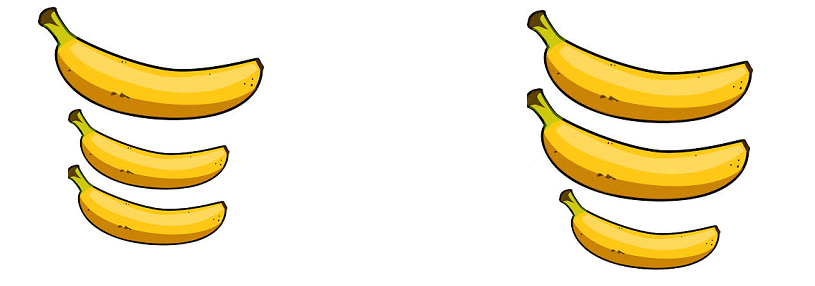
\includegraphics[height=0.15\textheight]{s03}

지수가 먹은 바나나 \qquad\qquad\quad 효정이가 먹은 바나나
\end{figure}

\ans

%
\prob
지수와 효정이는 바나나를 먹었습니다.
지수는 큰 바나나 2개를 먹었고 효정이는 큰 바나나 1개와 작은 바나나 3개를 먹었습니다.
지수와 효정이가 먹은 바나나의 양을 가장 간단한 자연수의 비로 나타내세요.
(단, 큰 바나나의 크기는 작은 바나나의 크기의 두 배입니다.)

\begin{figure}[h!]
\centering
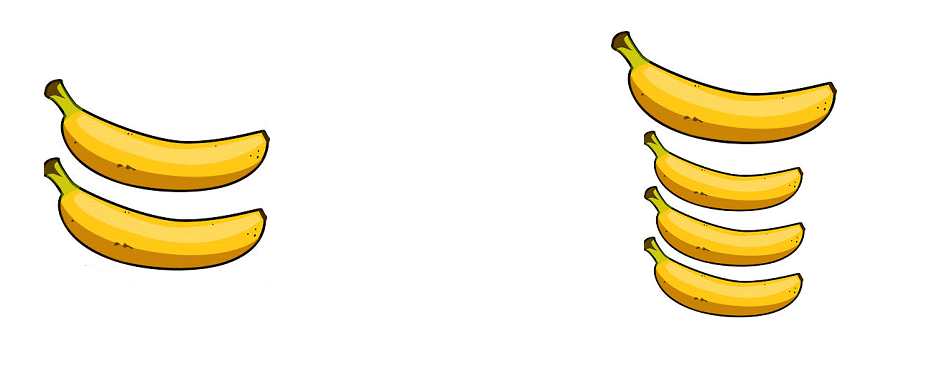
\includegraphics[height=0.19\textheight]{s04}

지수가 먹은 바나나 \qquad\qquad\quad 효정이가 먹은 바나나
\end{figure}

\ans
\end{document}